\chapter{Homology and bisimulations}
\label{chap:hombis}



Now we have all the ingredients for our directed homology theory: we have defined natural systems and bimodules of homology in Chapter 6, and we have specified how to compare those diagrams with bisimulations in Chapter 7. In the present chapter we will focus on the properties induced by comparing diagrams of homology with bisimilarity. First, as evoked several times earlier, we prove that natural systems and bimodules of homology are bisimilar in Section \ref{subsec:equibina}. We then investigate the relation between natural systems of homotopy and diagrams of homology by proving an analogue of Hurewicz theorem (Section \ref{subsec:dirhur}) and a first version of homotopy invariance (Section \ref{subsec:firhomax}).

From this point, we will restrict to a particular case, namely d-spaces that are geometric realization of cubical complexes, that is, spaces that are a finite union of some cubes in $\RR^n$. From this presentation of such a d-space, it will be possible to compute finite diagrams in modules by restricting natural systems of homology to some particular traces, obtained by concatenation of segments that join centers of cubes (Section \ref{subsec:distrahom}). We will prove in Sections \ref{subsec:funpar} and \ref{subsec:natisopar} that this finite diagram is bisimilar to the natural system of homology and from the work on the previous chapter, it will be decidable if two d-spaces which are geometric realizations of cubical complexes have bisimilar natural systems of homology. Finally, we relate this directed homology theory to the dihomotopy theory from Part II by proving in Section \ref{sec:sechomax} that two d-spaces which are the geometric realizations of cubical complexes and which are inessentially equivalent have bisimilar natural systems of homology.



\section{First easy consequences of using bisimulations}

\subsection{Equivalence of bimodules and natural systems}
\label{subsec:equibina}

First, we have defined two directed homologies: one using bimodules $\nathomolhm{n}{X}$, one using natural systems $\nathomolbw{n}{X}$. We have also seen that there is a functor $\map{\kappa_\C}{\fac{\C}}{\env{\C}}$ such that for every $n$, $$\nathomolbw{n}{X}\circ\kappa_{\trace{X}} = \nathomolhm{n}{X}.$$ 

\begin{prop}
$(\kappa_{\trace{X}}, \id)$ is an open map from $\nathomolbw{n}{X}$ to $\nathomolhm{n}{X}$. In particular, $\nathomolhm{n}{X}$ and $\nathomolbw{n}{X}$ are bisimilar for all $n$.
\end{prop}

\begin{proof}
Three properties to prove:
\begin{itemize}
	\item $\id$ is a natural isomorphism.
	\item $\kappa_\C$ is surjective on objects: let $(a,b)$ be an object of $\env{\C}$. This means that $a$ and $b$ are objects of $\C$ such that there is a morphism $f$ from $a$ to $b$. Then $f$ is an object of $\fac{\C}$ with $\kappa_\C(f) = (a,b)$.
	\item let $(\alpha,\beta)$ be a morphism from $(a,b)$ to $(a',b')$ in $\env{\C}$. This means that $\alpha$ is a morphism from $a'$ to $a$ and $\beta$ is a morphism from $b$ to $b'$ in $\C$. Let $f$ be such that $\kappa_\C(f) = (a,b)$. This means that $f$ is a morphism from $a$ to $b$ in $\C$. Consequently, $(\alpha,\beta)$ is a morphism from $f$ to $\beta\circ f \circ \alpha$ in $\fac{\C}$ and $\kappa_\C(\alpha,\beta) = (\alpha,\beta)$.
\end{itemize}
\end{proof}

\begin{prop}
\label{prop:nathomdim}
For every dimap $\map{f}{X}{Y}$, if $\nathomolbw{n}{f}$ is an open map, then $\nathomolhm{n}{f}$ is an open map.
\end{prop}

\begin{proof}
The natural morphism parts are the same, so if one is an isomorphism, the other is too.

For the functorial part, we prove the following more general statement. If $\map{F}{\C}{\D}$ is a functor, then if $\fac{F}$ satisfies the properties of an open map, that is, surjective on objects and the fibrational property, then $\env{F}$ satisfies them too. First, let us prove that $\env{F}$ is surjective on objects. Let $(c,d)$ be an object of $\env{\D}$. Then there is a morphism $f$ from $c$ to $d$. By surjectivity on objects of $\fac{F}$, there is a morphism $g$ from $a$ to $b$ with $\fac{F}(g) = F(g) = f$. In particular, $F(a) = c$ and $F(b) = d$, that is, $F(a,b) = (c,d)$. Next, let $(\alpha,\beta)$ be a morphism from $(c,d)$ to $(c',d')$ in $\env{\D}$ and let $a$, $b$ such that $F(a) = c$, $F(b) = d$ and $(a,b)$ being an object of $\env{\C}$. So there is a morphism $f$ from $a$ to $b$ in $\C$ and $(\alpha,\beta)$ is a morphism from $F(f)$ to $\beta\circ F(f)\circ \alpha$. By the fibrational property of $\fac{F}$, there is a morphism $(\alpha',\beta')$ in $\fac{\C}$ such that $F(\alpha') = \alpha$ and $F(\beta') = \beta$. $(\alpha',\beta')$ is also a morphism of $\env{\C}$.

We conclude by using this result on $\trace{f}$.
\end{proof}


\subsection{Directed Hurewicz theorem}
\label{subsec:dirhur}

Remember that Hurewicz theorem in classical algebraic topology states that homology in $\ZZ$-modules (i.e., Abelian groups) are deeply related to homotopy groups. We have the same here. In this subsection, we stick to directed homology in $\diagr{\Ab}$.

We say that a d-space $X$ is $1$-connected if $\nathomot{1}{X}$ is a diagram such that for every trace $\tra{\gamma}$, $\nathomot{1}{X}(\tra{\gamma})$ is a singleton, meaning that if $\gamma$ is a dipath from $a$ to $b$, $\tracep{X}{a}{b}$ has one connected components. For $n \geq 2$, we say that $X$ is $n$-connected if it is $n-1$ connected and if $\nathomot{n}{X}$ is a null diagram.

\begin{theo}[Directed Hurewicz theorem] Let $X$ be a d-space. Then:
\begin{itemize}
	\item $\nathomolbw{1}{X}$ is isomorphic to $\text{Free}\circ\nathomot{1}{X}$, where $\map{\text{Free}}{\setcat}{\Ab}$ is the functor that gives the free Abelian group generated by a set. $\nathomolhm{1}{X}$ is bisimilar to $\text{Free}\circ\nathomot{1}{X}$.
	\item if $X$ is $(n-1)$-connected, then:
		\begin{itemize}
			\item if $n =2$, $\nathomolbw{2}{X}$ is isomorphic to $\text{Abel}\circ\nathomot{2}{X}$, where $\map{\text{Abel}}{\group}{\Ab}$ is the functor that gives the abelianization of a group. $\nathomolhm{2}{X}$ is bisimilar to $\text{Abel}\circ\nathomot{2}{X}$.
			\item else, $\nathomolbw{n}{X}$ is isomorphic to $\nathomot{n}{X}$ and $\nathomolhm{n}{X}$ is bisimilar to $\nathomot{n}{X}$.
		\end{itemize}
\end{itemize}
\end{theo}

\begin{proof} This a consequence of the naturality of the classical Hurewicz theorem \end{proof}


\subsection{A first homotopy axiom}
\label{subsec:firhomax}

We have seen at the end of the Chapter 5 that we could state a homotopy axiom as follow: if a dimap induces isomorphisms between diagrams of homotopy then it induces isomorphisms between natural systems of homology. We then argued that isomorphisms are too strong and we develop the idea of bisimulations. The question now is: can we state a homotopy axiom using bisimulation ? Here is the answer:

\begin{theo}[First homotopy axiom]
Let $\map{f}{X}{Y}$ be a dimap. If for every $n$, $\map{\nathomot{n}{f}}{\nathomot{n}{X}}{\nathomot{n}{Y}}$ is an open map, then for every $n$, $\map{\nathomolbw{n}{f}}{\nathomolbw{n}{X}}{\nathomolbw{n}{Y}}$ and $\map{\nathomolhm{n}{f}}{\nathomolhm{n}{X}}{\nathomolhm{n}{Y}}$ are open maps.
\end{theo}

\begin{proof}
It is enough to prove it for natural systems by Proposition \ref{prop:nathomdim}.

The functorial parts of $\nathomot{n}{f}$ are the same as those of $\nathomolbw{n}{f}$. So if the parts of $\nathomot{n}{f}$ are surjective on objects and have the fibrational property, then those of $\nathomolbw{n}{f}$ too.

If the natural morphism part of $\nathomot{n}{f}$ is a isomorphism for every $n$, this means that for every pair $(a,b)$ such that there is a dipath from $a$ to $b$, the continuous function $$\map{\tracep{f}{a}{b}}{\tracep{X}{a}{b}}{\tracep{Y}{f(a)}{f(b)}}$$
which maps the trace $\tra{\gamma}$ to the trace $\tra{f\circ\gamma}$ induces a isomorphisms between homotopy groups for every $n$. So it induces isomorphisms between homology modules for every $n$, that is, the natural morphism part of $\nathomolbw{n}{f}$ is an isomorphism.
\end{proof}






\section{Cubical complexes}
\label{sec:cubcom}



Much as precubical sets, cubical complexes are finite unions of certain cubes of side-length
$1$ parallel to the axes in $\RR^d$, whose vertices have integer
coordinates \cite{kaczynskil03}.  Formally, let us define a
($d$-dimensional) \textbf{cubical complex} $K$ as a finite set of
\textbf{cubes} $(D, \vec x)$, where $D \subseteq \{1, 2, \cdots, d\}$
and $\vec x \in \ZZ^d$, which is closed under taking past and future
faces (to be defined shortly).  The cardinality $\lvert D \rvert$ of $D$ is the
\textbf{dimension} of the cube $(D, \vec x)$.  Let $\vec 1_k$ be the
$d$-tuple whose $k$th component is $1$, all others being $0$.  Each
cube $(D, \vec x)$ is \textbf{realized} as the geometric cube $\rho (D,
\vec x) = I_1 \times I_2 \times \cdots \times I_d$ where $I_k = [x_k,
x_k+1]$ if $k \in D$, $I_k = [x_k, x_k]$ otherwise, matching the
definition of \cite{kaczynskil03}.

When $\lvert D \rvert =n$, we write $D [i]$ for the $i$th element of $D$.  For
example, if $D = \{3, 4, 7\}$, then $D[1]=3$, $D[2]=4$, $D[3]=7$.  We
also write $\partial_i D$ for $D$ minus $D[i]$.  Every $n$-dimensional
cube $(D, \vec x)$ has $n$ \textbf{past faces} $\partial_i^0 (D, \vec
x)$, defined as $(\partial_i D, x)$, and $n$ \textbf{future faces}
$\partial_i^1 (D, \vec x)$, defined as $(\partial_i D, x + \vec
1_{D[i]})$, $1\leq i \leq n$.

Together with these face operators, $K$ exhibits the structure of a
precubical set. Cubical complexes are very particular
precubical sets. Notably, they are non-looping in the sense of \cite{fajstrup05}.  They are however enough for most purposes,
including the definition of geometric semantics of finite
SU/PV-programs.

The \textbf{geometric realization} $\digeom K$ of a precubical set $K$
is obtained using the study from Chapter \ref{chap:geomod}. It is the geometric realization using the functor from the category $\Box$ to the category $\dtop$ which maps $n$ to $\Box_n$ with the component-wise non-decreasing paths as dipaths (actually, everything could be done in any other category of directed spaces).


For example, the
matchbox is really obtained by drawing a
finite precubical set (a cubical complex, really) with $2$-dimensional
cubes $A$, $B$, $C$, $D$, and $E$, defined so that $\partial_1^0 A
= \partial_1^0 B$ (the lower dashed connection in the exploded view),
$\partial_2^0 A = a$, $\partial_2^0 B = b$, $\partial_1^0 a
= \partial_1^0 b = s$, and so on. 

Let us make this construction explicit here. Let $\overrightarrow\Box_n$
be the standard oriented cube $[0, 1]^n$, with dipaths the pointwise non-decreasing paths.
Form the coproduct $A = \sum_{e \in K} \overrightarrow \Box_{n_e}$ where
$n_e$ is the dimension of $e$, i.e., the disjoint union of as many
copies of $\overrightarrow \Box_n$ as there are $n$-dimensional cubes
$e$, for $n \in \nat$; the elements of $A$ are pairs $(e, \vec a)$
where $e$ is an $n$-dimensional cube in $K$ and $\vec a \in [0, 1]^n$,
for some $n$.  For convenience, for $\vec a = (a_1, a_2, \cdots,
a_n)$, we write $\delta_i^\alpha \vec a$ for $(a_1, a_2, \cdots,
a_{i-1}, \alpha, a_i, \cdots, a_n)$.  Finally, we glue all these cubes
together, by defining $\digeom K$ as $\quot A \equiv$, where $\equiv$
is the smallest equivalence relation such that $(\partial_i^\alpha e,
\vec a) \equiv (e, \delta_i^\alpha \vec a)$.  We shall write $[e, \vec
a]$ for the point obtained as the equivalence class of $(e, \vec a)$.


For a cubical complex $K$, the element $[(D, \vec x), \vec a]$ (with
$D \subseteq \{1, 2, \cdots, d\}$, $\lvert D \rvert=n$, $\vec x \in \ZZ^d$, $\vec a
\in [0, 1]^n$) of $\digeom K$ defines a point $\epsilon ([(D, \vec x),
\vec a]) = \vec x + \sum_{i=1}^n a_i \vec 1_{D [i]}$.  One checks
easily that $\epsilon$ is a dihomeomorphism of $\digeom K$ onto
the union of the cubes $\rho (D, \vec x)$, $(D, \vec x) \in K$.

The main interest of cubical complexes in our study is that from \cite{raussen12a}, the trace space of the geometric realization of a cubical complex is computable, in the sense that it is possible to compute a finite structure (namely a prod-simplicial complex) from which it is possible to compute homology modules. This will be a corner stone of computability of our directed homology.




\section{Discrete homology of a cubical complex}

\subsection{Discrete traces and homologies}
\label{subsec:distrahom}


Paralleling the notion of trace in a d-space, for example as in
\cite{fajstrup05}, there is a notion of \textbf{discrete trace} in a precubical
set $K$.  Given $a, b \in K$, say that $a$ is a \textbf{past boundary}
of $b$ if and only if $a = \partial_{i_0}^0 \partial_{i_1}^0
\cdots \partial_{i_k}^0 b$ for some $k \geq 0$, $i_0$, $i_1$, \ldots,
$i_k$.  \textbf{Future boundaries}
are defined similarly, using the superscript $1$ instead of $0$.  
We write $a \preceq b$ if and
only if $a$ is a past boundary of $b$ or $b$ is a future boundary of
$a$.  (Beware that this is not a transitive relation; we write
$\preceq^*$ for its reflexive transitive closure.)  A \textbf{discrete
  trace} from $a$ to $b$ in $K$ is then a sequence $c_0 = a \preceq
c_1 \preceq c_2 \preceq \cdots \preceq c_n = b$, $n \in \nat$.

Abusing the $\trace{X}$ notation we used earlier for d-spaces, let $\trace{K}$
be the small category whose objects are elements of $K$ and whose morphisms are discrete traces. Applying the enveloping category or factorization category constructions, gives us categories $\env{\trace{K}}$ and $\fac{\trace{K}}$. The objects of the first are pairs $(a,b)$ with $a \preceq^* b$, and the objects of the second are discrete traces. Their morphisms 
from a discrete trace from $a$ to $b$ to a discrete trace from $a'$ to $b'$ (or from $a \preceq^* b$ to $a' \preceq^* b'$)
are the \textbf{discrete extensions}, namely pairs of discrete
traces $\alpha$ from $a'$ to $a$ and $\beta$ from $b$ to $b'$.

Note that we are not restricting $a$, $b$ to be points, namely, of
dimension $0$; however, it is helpful to imagine, geometrically, that
a full cube $a$ stands for the point at its center.  The construction
is again due to Fajstrup \cite{fajstrup05}.  Formally, for $a = (D, \vec x)$,
$n = \lvert D \rvert$, let $\hat a$ be the point $[a, \bullet]$ in $\digeom K$,
where $\bullet = (\frac 1 2, \frac 1 2, \cdots, \frac 1 2)$ is the
center of the standard cube $\overrightarrow \Box_n$.  Through the
$\epsilon$ isomorphism, $\hat a$ is the point $\vec x + \sum_{i=1}^n
\frac 1 2 \vec 1_{D [i]}$ in $\RR^d$, the center of the cube $\rho
(D, \vec x)$.

Every discrete trace $\alpha$ from $a$ to $b$, say of the form $c_0 =
a \preceq c_1 \preceq c_2 \preceq \cdots \preceq c_n = b$, defines a
trace $\hat\alpha$ from $\hat a$ to $\hat b$, obtained by
concatenating the $n$ straight lines $\widehat {c_0 c_1}$, $\widehat
{c_1 c_2}$, \ldots, $\widehat {c_{n-1} c_n}$.  For a simple example,
consider the cubical complex whose geometric realization is shown on
Figure~\ref{fig:hat}, left.  There is a discrete trace $\alpha$ equal
to $b \preceq A \preceq t'$, since $b = \partial_1^0 A$ is a past
boundary of $A$ and $t' = \partial_2^1 \partial_1^1 A$ is a future
boundary of $A$.  The corresponding trace $\hat\alpha$ is shown on the
same figure, middle.  Formally, if $c_{i-1}$ is a past boundary
$\partial_{i_1}^0 \partial_{i_2}^0 \cdots \partial_{i_k}^0 c_i$ of
$c_i$, then $\hat c_{i-1} = [\partial_{i_1}^0 \partial_{i_2}^0
\cdots \partial_{i_k}^0 c_i, \bullet] = [c_i, \vec a]$ where $\vec a =
\delta_{i_k}^0 \cdots \delta_{i_2}^0 \delta_{i_1}^0 \bullet$; define
the dipath $\pi$ by $\pi (t) = [c_i, (1-t) \vec a + t \bullet]$ for $t
\in [0, 1]$, and the trace $\widehat {c_{i-1} c_i}$ as $\langle \pi
\rangle$.  Similarly for future boundaries.

\begin{figure}[H]
  % \vskip -.1cm
  \centering
    		  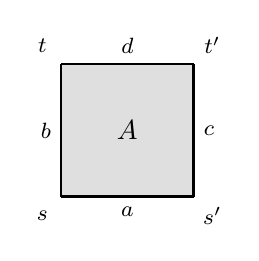
\begin{tikzpicture}[auto,scale = 1.2]
    \draw [fill = gray!25, draw = gray!75] (0,0) rectangle (1.4,1.4);
    \node (c) at (0.7,0.7) {$A$};
    \node   (x1) at (-0.2,-0.2) {\footnotesize{$s$}};
    \node  (x2) at (1.6,-0.2) {\footnotesize{$s'$}};
    \node  (x3) at (-0.2,1.6) {\footnotesize{$t$}};
    \node  (x4) at (1.6,1.6) {\footnotesize{$t'$}};
    \draw [thick] (0,0) to node [swap] {\footnotesize{$a$}} (1.4,0);
    \draw [thick] (0,0) to node {\footnotesize{$b$}} (0,1.4);
    \draw [thick] (1.4,0) to node [swap] {\footnotesize{$c$}} (1.4,1.4);
    \draw [thick] (0,1.4) to node {\footnotesize{$d$}} (1.4,1.4);
  \end{tikzpicture}
  \qquad
  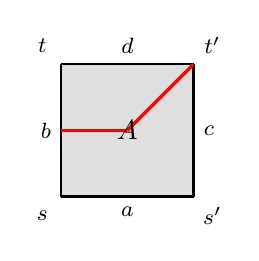
\begin{tikzpicture}[auto,scale = 1.2]
    \draw [fill = gray!25, draw = gray!75] (0,0) rectangle (1.4,1.4);
    \draw [thick] (0,0) to node [swap] {\footnotesize{$a$}} (1.4,0);
    \draw [thick] (0,0) to node {\footnotesize{$b$}} (0,1.4);
    \draw [thick] (1.4,0) to node [swap] {\footnotesize{$c$}} (1.4,1.4);
    \draw [thick] (0,1.4) to node {\footnotesize{$d$}} (1.4,1.4);
    \draw [very thick,red] (0,0.7) to (0.7,0.7);
    \draw [very thick,red] (0.7,0.7) to (1.4,1.4);
    \node (c) at (0.7,0.7) {$A$};
    \node   (x1) at (-0.2,-0.2) {\footnotesize{$s$}};
    \node  (x2) at (1.6,-0.2) {\footnotesize{$s'$}};
    \node  (x3) at (-0.2,1.6) {\footnotesize{$t$}};
    \node  (x4) at (1.6,1.6) {\footnotesize{$t'$}};
  \end{tikzpicture}
  \qquad
  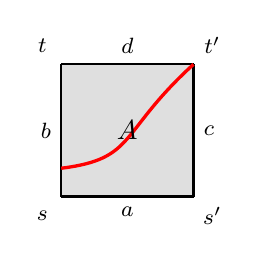
\begin{tikzpicture}[auto,scale = 1.2]
    \draw [fill = gray!25, draw = gray!75] (0,0) rectangle (1.4,1.4);
    \draw [thick] (0,0) to node [swap] {\footnotesize{$a$}} (1.4,0);
    \draw [thick] (0,0) to node {\footnotesize{$b$}} (0,1.4);
    \draw [thick] (1.4,0) to node [swap] {\footnotesize{$c$}} (1.4,1.4);
    \draw [thick] (0,1.4) to node {\footnotesize{$d$}} (1.4,1.4);
    \draw[red,very thick] (0,0.3) .. controls (0.8,0.4) and (0.6,0.67) .. (1.4,1.4);
    \node (c) at (0.7,0.7) {$A$};
    \node   (x1) at (-0.2,-0.2) {\footnotesize{$s$}};
    \node  (x2) at (1.6,-0.2) {\footnotesize{$s'$}};
    \node  (x3) at (-0.2,1.6) {\footnotesize{$t$}};
    \node  (x4) at (1.6,1.6) {\footnotesize{$t'$}};
  \end{tikzpicture}
  \caption{From discrete traces to traces and vice versa}
  \label{fig:hat}
\end{figure}

$\widehat{~.~}$ then defines a functor from $\trace{K}$ to $\trace{\digeom{K}}$. We can define the \textbf{$n$th discrete bimodule of homology of $K$} as the functor 
$$\map{\disnathomolhm{n}{K}}{\env{\trace{K}}}{\modu{\R}} = \overrightarrow{DBH}_{n}\circ\env{\widehat{~.~}}.$$
Similarly, one can define the \textbf{$n$th discrete natural system of homology of $K$} as the functor
$$\map{\disnathomolbw{n}{K}}{\fac{\trace{K}}}{\modu{\R}} = \overrightarrow{DBH}_{n}\circ\fac{\widehat{~.~}}.$$
As in the case of d-spaces, there is an open map from $\disnathomolbw{n}{K}$ to $\disnathomolhm{n}{K}$, and so, the two constructions are bisimilar.

Discrete homologies are constructed by considering only a finite number of homology modules of trace spaces, while homologies of the geometric realization are (in general) not even countable. That does make a difference up to isomorphisms, not up to bisimulation:

\begin{theo}[Discrete Homology$\equiv$Geometric Homology]
\noindent For every cubical complex $K$, there is an open map from $\nathomolbw{n}{\digeom{K}}$ to $\disnathomolbw{n}{K}$.  In particular, $\nathomolbw{n}{\digeom{K}}$, $\nathomolhm{n}{\digeom{K}}$, $\disnathomolbw{n}{K}$ and $\disnathomolhm{n}{K}$ are all bisimilar.
\end{theo}

The next subsections are dedicated to the construction of the open map $(\carrier,\sigma)$ from $\nathomolbw{n}{\digeom{K}}$ to $\disnathomolbw{n}{K}$.


\subsection{Construction of the functorial part}
\label{subsec:funpar}

In this Section, we assume that $K$ is a cubical complex, and $X$ is
its geometric realization $\digeom K$.

  The functor $\carrier$ is based on the notion of \textbf{carrier sequence} due to
  Fajstrup \cite{fajstrup05}.  For a point $s$ in $X$, there is a
  unique cube $e \in K$ of minimal dimension $m$ such that $s$ can be
  written as $[e, \vec a]$, $\vec a \in \overrightarrow \Box_m$.  Write
  $\carrier (s)$ for this cube $e$, and call it the \textbf{carrier}
  of $s$.  Every trace $\tra{\gamma}$ in $X$ gives rise to an
  ordered sequence of cubes $\carrier(\tra{\gamma})$
  obtained as the carriers of $\gamma (t)$, $t \in [0, 1]$, and removing
  consecutive duplicates.  More precisely, given a dipath $\gamma$ of $X$, there is
a unique sequence $c_0,c_1,\cdots,c_k$ of elements of $K$ and a unique
sequence of real numbers $0=t_0\leq t_1\leq\cdots\leq t_k \leq
t_{k+1}=1$ (call them the \textbf{times of change}) such that:
\begin{itemize}
\item for every $1\leq i \leq k$, $c_{i-1} \neq c_i$,
\item for every $0\leq i\leq k$, for every $t \in [t_i,t_{i+1}]$, $\gamma
  (t)$ is a point of the form $[c, \vec a]$ with $c=c_i$,
\item for every $0\leq i \leq k$, for every $t\in (t_i,t_{i+1})$,
  $\carrier(\gamma(t)) = c_i$,
\item $\carrier(\gamma(0)) = c_0$ and $\carrier(\gamma(1)) = c_k$,
\item for every $1\leq i \leq k$, $\carrier(\gamma(t_i)) \in
  \{c_{i-1},c_i\}$ and if furthermore $t_i = t_{i+1}$ then
  $\carrier(\gamma(t_i)) = c_i$.
\end{itemize}
The sequence $c_0,c_1,\cdots,c_k$ is called the \textbf{carrier sequence of
  $\gamma$}.  Two dipaths that are equivalent modulo reparametrization
have the same carrier sequence, so it is legitimate to call carrier
sequence, $\carrier(\gamma)$ of $\gamma$ the carrier sequence of the trace, $\tra{\gamma}$, of $\gamma$. By a compactness argument $\carrier(\tra{\gamma})$ is a finite
  sequence, in fact a discrete trace. For example, the carrier
  sequence of the trace on the right of Figure~\ref{fig:hat} is $b
  \preceq A \preceq t'$.
  
  We use this to define our functor $\carrier$, on objects by
  letting $\carrier(\tra{\gamma})$ be defined as above, 
  and on morphisms by letting $\carrier(\tra{\alpha},\tra{\beta}) = (\carrier(\tra{\alpha}),\carrier(\tra{\beta}))$ for every extension
  $(\tra{\alpha},\tra{\beta})$.  This
  is surjective on objects since $\carrier (\hat \gamma) = \gamma$ for every
  discrete trace $\gamma$.  We now claim that $\carrier$ is the functorial part of an open map, and this
  amounts to show that: given any trace $\tra{\gamma}$ of
  $\digeom{K}$, with carrier sequence $c_0 \preceq \cdots \preceq c_k$, if the
    latter extends to a discrete trace $c_{-p} \preceq \cdots \preceq
    c_{-1} \preceq c_0 \preceq \cdots \preceq c_k \preceq c_{k+1}
    \preceq \cdots \preceq c_{k+q}$ in $K$, then $\tra{\gamma}$
    extends to some trace $\tra{\alpha \star \gamma \star \beta}$ such that $\carrier(\tra{\alpha \star \gamma \star \beta}) =
    c_{-p} \preceq \cdots \preceq c_{-1} \preceq c_0 \preceq \cdots
    \preceq c_k \preceq c_{k+1} \preceq \cdots \preceq c_{k+q}$.  By
    induction, the cases $(p,q)=(1,0)$ and $(p,q)=(0,1)$ suffice to
    establish the property.  Some care has to be taken: the extension
    paths are \emph{not} concatenations of simple straight lines
    joining the extra points $\hat c_j$, $j \geq k$ or $j\leq 0$.  As
    the following shows (for $(p,q)=(0,2)$),
    
    \begin{figure}[H]
  % \vskip -.1cm
  \centering
    		    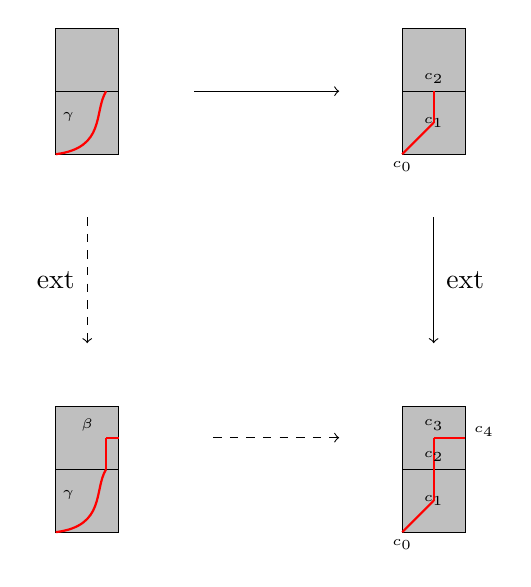
\begin{tikzpicture}[scale = 0.8]
      \draw[fill = gray!50] (0,0) rectangle (1,1);
      \draw[fill = gray!50] (0,1) rectangle (1,2);
      \draw[red,thick] (0,0) .. controls (0.8,0.1) and (0.6,0.67) .. (0.8,1);
      \node at (0.2,0.6) {\tiny$\tra{\gamma}$};
      \draw[->] (2.2,1) -- (4.5,1);
      \node at (3.5,1.3) {$\carrier$};
      \draw[fill = gray!50] (5.5,0) rectangle (6.5,1);
      \draw[fill = gray!50] (5.5,1) rectangle (6.5,2);
      \draw[red,thick] (5.5,0) -- (6,0.5);
      \draw[red,thick] (6,0.5) -- (6,1);
      \node at (5.5,-0.2) {\tiny$c_0$};
      \node at (6,0.5) {\tiny$c_1$};
      \node at (6,1.2) {\tiny$c_2$};
      \draw[->] (6,-1) -- (6,-3);
      \node at (6.5,-2) {ext};
      \draw[fill = gray!50] (5.5,-6) rectangle (6.5,-5);
      \draw[fill = gray!50] (5.5,-5) rectangle (6.5,-4);
      \draw[red,thick] (5.5,-6) -- (6,-5.5);
      \draw[red,thick] (6,-5.5) -- (6,-5);
      \draw[red,thick] (6,-5) -- (6,-4.5);
      \draw[red,thick] (6,-4.5) -- (6.5,-4.5);
      \draw[->,dashed] (0.5,-1) -- (0.5,-3);
      \node at (5.5,-6.2) {\tiny$c_0$};
      \node at (6,-5.5) {\tiny$c_1$};
      \node at (6,-4.8) {\tiny$c_2$};
      \node at (6, -4.3) {\tiny$c_3$};
      \node at (6.8, -4.4) {\tiny$c_4$};
      \node at (0,-2) {ext};
      \draw[fill = gray!50] (0,-6) rectangle (1,-5);
      \draw[fill = gray!50] (0,-5) rectangle (1,-4);
      \draw[red,thick] (0,-6) .. controls (0.8,-5.9) and (0.6,-5.33) .. (0.8,-5);
      \draw[red,thick] (0.8,-5) -- (0.8,-4.5);
      \draw[red,thick] (0.8,-4.5) -- (1,-4.5);
      \node at (0.2,-5.4) {\tiny$\tra{\gamma}$};
      \node at (0.5,-4.3) {\tiny$\tra{\beta}$};
      \draw[->,dashed] (2.5,-4.5) -- (4.5,-4.5);
      \node at (3.5,-4.1) {$\carrier$};
    \end{tikzpicture}
\end{figure}
   \noindent the dipath
    $\beta$ does not---and cannot---go through $\hat c_3$. 
    Details of the construction are given by the following lemma:
    
    \begin{lemme}
  \label{lemma:bisim:C}
  Let $\tra{\gamma}$ be a trace in $X$ ($=\digeom K$) with
  carrier sequence $c_0 \preceq c_1 \preceq \cdots \preceq c_k$.
  \begin{itemize}
  \item For every cube $c_{-1} \preceq c_0$, there is a dipath
    $\alpha$ in $X$ such that
    $\carrier(\tra{\alpha\star\gamma}) = c_{-1} \preceq c_0
    \preceq c_1 \preceq \cdots \preceq c_k$.
  \item For every cube $c_{k+1}$ such that $c_k \preceq c_{k+1}$,
    there is a dipath $\beta$ in $X$ such that $\carrier(\tra{
    \gamma \star \beta}) = c_0 \preceq c_1 \preceq \cdots \preceq
    c_k \preceq c_{k+1}$.
  \end{itemize}
\end{lemme}


\begin{proof}
  We examine the second case only: the other case is symmetric.  Since
  $c_k \preceq c_{k+1}$, $c_k$ can be a past boundary of $c_{k+1}$, or
  $c_{k+1}$ can be a future boundary of $c_k$.  We examine both cases:
  \begin{itemize}
  \item If $c_k$ is a past boundary of $c_{k+1}$, say $c_k
    = \partial_{i_p}^0\cdots\partial_{i_0}^0 c_{k+1}$, then by using
    the precubical equations we may require $i_0 > \ldots > i_p$.
    Writing $\gamma(1)$ as $[c_k, \vec a]$, we also have $\gamma (1) =
    [c_{k+1}, \delta_{i_0}^0 \cdots \delta_{i_p}^0 \vec a]$ by the
    definition of the geometric realization.  Since $\carrier(\gamma
    (1)) = c_k$, no component $a_i$ of $\vec a$ is equal to $0$ or
    $1$.  Let $\vec b = \delta_{i_0}^0 \cdots \delta_{i_p}^0 \vec a$:
    it follows that the components $b_i$ of $\vec b$ that are equal to
    $0$ are exactly those such that $i\in\{i_0,\cdots,i_p\}$.  Let
    $\vec a'$ be the tuple whose $i$th component $a'_i$ is $1/2$ if
    $b_i=0$, and $b_i$ otherwise.  We define the dipath $\beta$ by
    $\beta (t) = [c_{k+1},(1-t) \vec b +t \vec a')]$, $t \in [0, 1]$.
    Note that $\beta$ is indeed monotonic, because $b_i \leq a'_i$ for
    every $i$.  One easily checks that $\beta (0) = \pi (1)$, and that
    the carrier sequence of $\tra{\beta}$ is $c_k \preceq
    c_{k+1}$: for $t=0$, $\carrier(\beta (0)) = \carrier(\gamma (1))
    = c_k$, and, for $t \neq 0$, $\beta (t) = [c_{k+1},(1-t) \vec b +t
    \vec a')]$ where no component of $(1-t) \vec b +t \vec a'$ is
    equal to $0$ or $1$, so its carrier $\carrier (\beta (t))$ is
    $c_{k+1}$.  It follows that
    $\carrier(\tra{\gamma\star\beta}) = c_0 \preceq c_1
    \preceq \cdots \preceq c_k \preceq c_{k+1}$.
  \item If $c_{k+1}$ is a future boundary of $c_k$, then $c_{k+1}$ is
    of the form $\partial_{i_p}^1\ldots\partial_{i_0}^1 c_k$ with $i_0
    > \ldots > i_p$, and $\gamma (1) = [c_k, \vec a]$ for some tuple
    $\vec a$ whose components $a_i$ are all different from $0$ or $1$
    (because $\carrier(\gamma (1)) = c_k$).  Let $\vec b$ be the tuple
    obtained from $\vec a$ by changing the $i$th component into $1$
    if and only if $i \in \{i_0, \cdots, i_p\}$.  In other words, let
    $b_i = 1$ if $i \in \{i_0, \cdots, i_p\}$, $b_i=a_i$ otherwise.
    One can therefore write $\vec b$ as $\delta_{i_0}^1 \cdots
    \delta_{i_p}^1 \vec b'$, where $\vec b'$ is the tuple obtained
    from $\vec b$ by removing its components of indices $i_0$, \ldots,
    $i_p$.  Define the dipath $\beta$ by $\beta (t) = [c_k, (1-t) \vec
    a + t \vec b]$.  This is monotonic because $a_i \leq b_i$ for
    every $i$.  For $t \neq 1$, no component of $(1-t) \vec a + t \vec
    b$ is equal to $0$ or $1$, so $\carrier(\beta (t))=c_k$, and
    for $t=1$, $\beta (1) = [c_k, \vec b] = [c_{k+1}, \vec b']$, which
    shows that $\carrier(\beta (1)) = c_{k+1}$ since no component
    of $\vec b'$ is equal to $0$ or $1$.  Again, it follows that
    $\carrier(\tra{\gamma\star\beta}) = c_0 \preceq c_1
    \preceq \cdots \preceq c_k \preceq c_{k+1}$. 
  \end{itemize}
\end{proof}



\subsection{Construction of the natural isomorphism part}
\label{subsec:natisopar}


We now need to build a natural isomorphism
  $\map{\sigma}{\overrightarrow{NH}_{n}}{\overrightarrow{DNH}_n\circ\carrier}$.  In other words, we need to build
  isomorphisms of modules $\map{\sigma_{\tra{\gamma}}}{H_n(\tracep{X}{a}{b})}{H_n(\tracep{X}{\carrier(a)}{\carrier(b)})}$ for $\gamma$ a dipath from $a$ to $b$, that are natural, in the sense that, for every extension $(\tra{\alpha},\tra{\beta})$ of $\tra{\gamma}$, with $\alpha$ a dipath from $a'$ to $a$ and $\beta$ a dipath from $b$ to $b'$, the following square commutes:
\begin{figure}[H]
  % \vskip -.1cm
  \centering
    		
    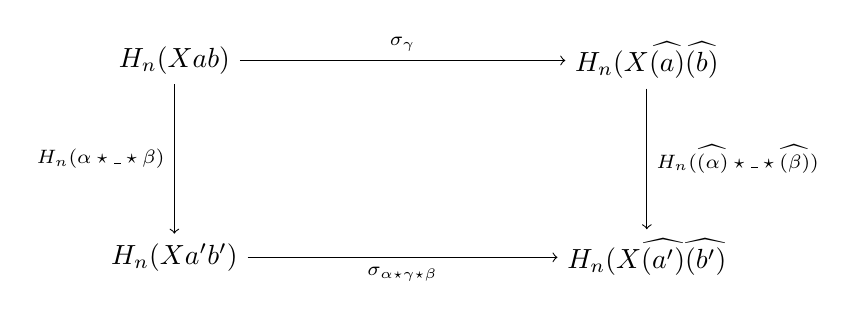
\begin{tikzpicture}
      \node (Fx') at (1,0) {$H_n(\tracep{X}{a'}{b'})$};
      \node (Fx) at (1,2.5) {$H_n(\tracep{X}{a}{b})$};
      \node (Gy') at (7,0) {$H_n(\tracep{X}{\widehat{\carrier(a')}}{\widehat{\carrier(b')}}$};
      \node (Gy) at (7,2.5) {$H_n(\tracep{X}{\widehat{\carrier(a)}}{\widehat{\carrier(b)}}$};
      \path[->,font=\scriptsize] 
      		(Fx) edge node[left]{$H_n(\tra{\alpha \star \_ \star \beta})$} (Fx')
      		(Fx) edge node[above]{$\sigma_{\tra{\gamma}}$} (Gy)
      		(Fx') edge node[below]{$\sigma_{\tra{\alpha\star\gamma\star\beta}}$} (Gy')
      		(Gy) edge node[right]{$H_n(\tra{\widehat{\carrier(\alpha)} \star \_ \star \widehat{\carrier(\beta)}})$} (Gy');
    \end{tikzpicture}
\end{figure}
\noindent where $\tra{\alpha\star\_\star\beta}$ is the continuous function which maps the trace $\tra{\rho}$ to the trace $\tra{\alpha\star\rho\star\beta}$.

Let $\gamma$ be from $s$ to $t$. Every cube $\Box_k$ has a lattice structure whose meet $\wedge$ is
    pointwise $\min$ and whose join $\vee$ is pointwise $\max$.  Write
    $s$ as $[\carrier(s), \vec a]$, and let $s_- = [\carrier(s),
    \vec a \wedge \bullet]$.  Recall that $\bullet = (\frac 1 2,
    \cdots, \frac 1 2)$, and that $\widehat {\carrier(s)} =
    [\carrier(s), \bullet]$.  Similarly, let $\widehat {\carrier
      (t)} = [\carrier(t), \bullet]$, and we define $t_+ =
    [\carrier(t), \vec b \vee \bullet]$, where $t = [\carrier(t), \vec b]$.  The situation is illustrated here:
    \begin{figure}[H]
  % \vskip -.1cm
  \centering
    		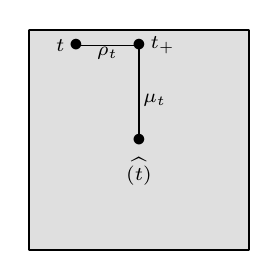
\begin{tikzpicture}[auto, scale = 2]
      \draw [fill = gray!25, draw = gray!75] (0,0) rectangle (1.4,1.4);
      \draw [thick] (0,0) -- (1.4,0);
      \draw [thick] (0,0) -- (0,1.4);
      \draw [thick] (1.4,0) -- (1.4,1.4);
      \draw [thick] (0,1.4) -- (1.4,1.4);
      \node (s-) at (0.7,1.3) {$\bullet$};
      \node at (0.85,1.3) {\scriptsize{$t_+$}};
      \node (s) at (0.3,1.3) {$\bullet$};
      \node at (0.2,1.3) {\scriptsize{$t$}};
      \node (hs) at (0.7,0.7) {$\bullet$};
      \node at (0.7,0.5) {\scriptsize{$\widehat {\carrier(t)}$}};
      \draw (0.7,1.3) -- (0.7,0.7);
      \draw (0.7,1.3) -- (0.3,1.3);
      \node at (0.8,0.95) {\scriptsize{$\mu_t$}};
      \node at (0.5,1.25) {\scriptsize{$\rho_t$}};
    \end{tikzpicture}
    \qquad\qquad
    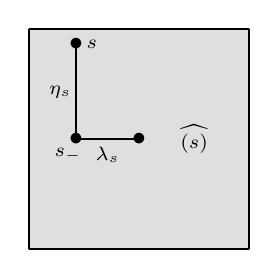
\begin{tikzpicture}[auto,scale = 2]
      \draw [fill = gray!25, draw = gray!75] (0,0) rectangle (1.4,1.4);
      \draw [thick] (0,0) -- (1.4,0);
      \draw [thick] (0,0) -- (0,1.4);
      \draw [thick] (1.4,0) -- (1.4,1.4);
      \draw [thick] (0,1.4) -- (1.4,1.4);
      \node (s-) at (0.3,0.7) {$\bullet$};
      \node at (0.25,0.6) {\scriptsize{$s_-$}};
      \node (s) at (0.3,1.3) {$\bullet$};
      \node at (0.4,1.3) {\scriptsize{$s$}};
      \node (hs) at (0.7,0.7) {$\bullet$};
      \node at (1.05,0.7) {\scriptsize{$\widehat {\carrier(s)}$}};
      \draw (0.3,0.7) -- (0.7,0.7);
      \draw (0.3,0.7) -- (0.3,1.3);
      \node at (0.5,0.6) {\scriptsize{$\lambda_s$}};
      \node at (0.2,1.0) {\scriptsize{$\eta_s$}};
    \end{tikzpicture}
\end{figure}
    

    There are obvious dipaths $\eta_s$, $\lambda_s$, $\mu_t$, $\rho_t$
    as displayed there, too. For example, $\eta_s (t) = [\carrier(s), (1-t) (\vec a
\wedge \bullet) + t \vec a]$. Those induce continuous maps between
    trace spaces by concatenation. For example, there is a continuous map
$\map{\eta_s^*}{\tracep{X}{s}{t}}{\tracep{X}{s_-}{t}}$ that sends each
trace $\tra{\pi}$ to $\tra{\eta_s\star\pi}$.
Similarly, $\lambda_s^* (\tra{\pi}) = \tra{\lambda_s
\star \pi}$, and symmetrically, ${^*\mu_t} (\tra{\pi}) = \tra{\pi \star \mu_t}$, ${^*\rho_t} (\tra{\pi}) = \tra{\pi \star \rho_t}$. We prove now that all those continuous functions are homotopy equivalences. The proof will use the following technical lemma:

\begin{lemme}
\label{lem:tech}
  Let $\map{F,G}{\dipp{X}{s}{t}}{\dipp{X}{s'}{t'}}$ such that:
  \begin{itemize}
  \item for every pair of dipaths $\gamma$, $\rho$ that are equivalent modulo
    reparametrization, $F(\gamma)$ and $F(\rho)$ are equivalent modulo
    reparametrization---so $F$ induces
    $\map{\tilde{F}}{\tracep{X}{s}{t}}{\tracep{X}{s'}{t'}}$, and
    similarly for $G$.
  \item for every $\gamma$, $F(\gamma)$ and $G(\gamma)$ have the same carrier sequence.
  \end{itemize}
  Then $\tilde{F}$ and $\tilde{G}$ are homotopic.
\end{lemme}

\begin{proof}
  Let $C(X)(s',t')$ be the subspace of $\dipp{X}{s'}{t'}\times\dipp{X}{s'}{t'}$
  that consists of pairs of dipaths that have the same carrier
  sequence. The key ingredient consists in constructing a continuous
  map $\map{\Gamma}{[0,1]\times C(X)(s',t')}{\dipp{X}{s'}{t'}}$ in such a way
  that $\Gamma (0, (p, q)) = p$ and $\Gamma (1, (p, q)) = q$.  Let
  $c_0, c_1, \cdots, c_k$ be the common carrier sequence to $p$ and
  $q$, let $t_0\leq t_1 \leq \cdots\leq t_{k+1}$ be the times of
  change for $p$, and $s_0 \leq s_1 \leq \cdots \leq s_{k+1}$ be the
  times of change for $q$.  Define $u_i (t) = ts_i + (1-t)t_i$ for $t
  \in [0, 1]$, $0\leq i\leq k+1$.  For every $u \in [u_i(t),
  u_{i+1}(t)]$, define $v$ as $\frac{u-u_i(t)}{u_{i+1}(t)-u_i(t)}$.
  (This is defined provided $u_i(t)\neq u_{i+1}(t)$; if this is not
  the case, let $v=0$.)  Then $p(v(t_{i+1}-t_i) + t_i)$ is of the form
  $[c_i,(a_1^u,\ldots,a_m^u)]$ and $q(v(s_{i+1}-s_i) + s_i)$ is of the
  form $[c_i,(b_1^u,\ldots,b_m^u)]$. We then define $\Gamma(t,p,q)(u)
  = [c_i,(1-t)a_j^u+tb_j^u]$.

  We have to define a homotopy
  $\map{H}{[0,1]\times\tracep{X}{s}{t}}{\tracep{X}{s'}{t'}}$. It will be
  defined as the composition of:
  \begin{itemize}
  \item $\map{\id\times \kappa}{[0,1]\times\tracep{X}{s}{t}}{[0,1]\times
      \dipp{X}{s}{t}}$, where $\kappa$ is a continuous map from $\tracep X s
    t$ to $\dipp{X}{s}{t}$, defined in such a way that $\tra{\kappa(\tra{\pi})} = \tra{\pi}$ for every
    trace $\tra{\pi}$, therefore defining a canonical dipath
    representing a given trace.  The existence of such a map is shown
    by Raussen in \cite{raussen09}, as the composition
    $\text{norm}\circ\overrightarrow{s}$ of two more elementary maps.
  \item $\map{\id\times(F, G)}{[0,1]\times \dipp{X}{s}{t}}{[0,1]\times C(X)(s',t')}$,
    where $(F, G)$ maps $\pi$ to $(F (\pi), G (\pi))$.
  \item $\map{\Gamma}{[0,1]\times C(X)(s',t')}{\dipp{X}{s'}{t'}}$, as defined above.
  \item and $\map{\tra{\_}}{\dipp{X}{s'}{t'}}{\tracep{X}{s'}{t'}}$,
    which maps each dipath to its trace.
  \end{itemize}
  We compute: $H(0,\tra{\pi}) = \tra{\Gamma (0, (F
  (\kappa (\tra{\pi})), G (\kappa (\tra{\pi})))} = \tra{ F(\kappa (\tra{\pi})) } =
  \tilde{F}(\tra{\pi})$.  Similarly, $H(1,\_) = \tilde{G}$
  and therefore $H$ is a homotopy from $\tilde{F}$ to $\tilde{G}$.
\end{proof}

\begin{lemme}
\label{lem:tech2}
  The maps $\eta_s^*$, $\lambda_s^*$, ${^*\mu_t}$ and ${^*\rho_t}$ are homotopy equivalences.
\end{lemme}

\begin{proof}
  We prove it for $\eta_s^*$, the other three being similar. By abuse of language, write $\eta_s^* (\pi)$ for the dipath $\eta_s
  \star \pi$ as well---we reason on spaces of dipaths first, then take
  a reparametrization quotient.  

  Observe that $\eta_s^*$ maps $\dipp{X}{s}{t}$ to $\dipp{X}{s_-}{t}$.  We
  need to build a map $\map{\nu}{\dipp{X}{s_-}{t}}{\dipp{X}{s}{t}}$ such that
  $\eta_s^* \circ \tilde{\nu}$ and $\tilde{\nu} \circ \eta_s^*$ are homotopic to the
  identity using the previous lemma.

  For every dipath $\pi$ from $s$ to $t$, the carrier sequence $c_0,
  c_1, \cdots,c_k$ of $\eta_s^* (\pi)$ is equal to that of $\pi$.
  In the other direction, we shall define $\nu$ so that it also
  preserves the carrier sequence.  This will turn out to be the
  crucial property that will allow us to conclude by the previous lemma.

  For every dipath $\pi$ from $s_-$ to $t$, with carrier sequence
  $c_0, c_1, \cdots, c_k$, and with times of change $0=t_0\leq
  t_1\leq\cdots\leq t_k \leq t_{k+1}=1$, we define $\nu (\pi)$ as follow.  We
  abuse the notation $\vee$, and write $[c, \vec a] \vee_c [c, \vec
  b]$ for $[c, \vec a \vee \vec b]$.  The three occurrences of $c$
  must be the same for this notation to make sense, but our intuition
  is best served by ignoring the $c$ subscript to $\vee$, and to
  understand this as taking maxes, componentwise, in a local cube $c$.
  We then define $\nu (\pi) (u)$ for increasing values of $u$,
  inductively, as $s \vee_{c_0} \pi (u)$ for $u \in [t_0, t_1]$, as
  $\nu (\pi) (t_1) \vee_{c_1} \pi (u)$ for $u \in [t_1, t_2]$, \ldots,
  and finally as $\nu (\pi) (t_k) \vee_{c_k} \pi (u)$ for $u \in [t_k, t_{k+1}]$.

  On $[t_0, t_1]$, $\nu (\pi)$ is a continuous monotonic map, with
  value $\nu (\pi) (0) = s \vee_{c_0} s_- = s$ at $u=t_0=0$, and with
  value $\nu (\pi) (t_1) = s \vee_{c_0} \pi (t_1)$ at $u=t_1$.
  
  Let us show by induction on $j$ that for every $u$ with $0 \leq
  u\leq t_j$, $\carrier(\nu(\pi)(u)) = \carrier(\pi(u))$. For $j
  = 0$, this says that $\carrier(s) = \carrier(s_-)$, which is
  by construction of $s_-$.  Otherwise, by induction hypothesis, for
  every $u$ with $0 \leq u\leq t_j$, $\carrier(\nu(\pi)(u)) =
  \carrier(\pi(u))$. Let $t_j < u \leq t_{j+1}$.  We can write
  $\pi(t_j)$ as $[c_j,(b_1,\ldots,b_m)]$ and $\pi (u)$ as
  $[c_j,(a_1,\ldots,a_m)]$, where $b_i \leq a_i$ for every $i$.
  \begin{itemize}
  \item If $u < t_{j+1}$, by the properties of the carrier sequence,
    $\carrier(\pi(u)) = c_j$, so with $0 < a_i < 1$ for every $i$.
    Since $b_i \leq a_i$, $b_i < 1$ for every $i$.  Let us write
    $\nu(\pi)(t_j)$ as $[c_j,(b'_1,\ldots,b'_m)]$.  Since
    $\carrier(\nu(\pi)(t_j)) = \carrier(\pi(t_j))$, $b_i = 1$
    iff $b'_i = 1$.  It follows that $b'_i < 1$ for every $i$.
    Therefore $0 < \max(a_i,b'_i) < 1$, so $\carrier(\nu(\pi)(u)) =
    c_k$.
  \item If $u = t_{j+1}$, we observe that $\max (a_i, b'_i)$ is equal
    to $1$, resp.\ to $0$, resp.\ in $(0, 1)$, if and only if $a_i$
    is.  This observation is enough to conclude that
    $\carrier(\nu(\pi)(t_{j+1})) = \carrier(\pi(t_{j+1}))$, and
    is proved as follows.  If $a_i = 1$, then $\max(a_i, \allowbreak
    b'_i) = 1$. If $a_i = 0$ then $b_i = 0$; moreover, since
    $\carrier(\nu(\pi)(t_j)) = \carrier(\pi(t_j))$, $b_i = 0$
    iff $b'_i = 0$, so $b'_i = 0$, from which we obtain
    $\max(a_i,b'_i) = 0$.  Finally, if $0 < a_i < 1$ then $b_i < 1$,
    and $b'_i < 1$ (since $\carrier(\nu(\pi)(t_j)) =
    \carrier(\pi(t_j))$, $b_i = 1$ iff $b'_i = 1$), so $0 <
    \max(a_i,b'_i) < 1$.
  \end{itemize}
  This finishes our argument that $c_0,\ldots,c_k$ is the carrier
  sequence of $\nu(\pi)$, with times of change $0=t_0\leq \ldots \leq
  t_{k+1}=1$.
  
  It remains to show that $\nu(\pi)(1) = t$.  This is the only place
  where we need the $\epsilon$ mapping.  The above argument works in
  general precubical sets, not just cubical complexes.  On the
  contrary, we need the specific features of cubical complexes to show
  that $\nu (\pi) (1)=t$.  We discuss this in a remark at the end of
  the section.

  We know that $\carrier(t) = \carrier(\nu(\pi)(1)) = c_k$.
  Moreover, $t$ is below $\nu(\pi)(1)$ in the ordering $\leq$ of the
  pospace $X = \digeom K$, because $\nu(\pi)(1) = \nu(\pi)(t_k)
  \vee_{c_k} \pi(1) = \nu(\pi)(t_k) \vee_{c_k} t$. Suppose that
  $\nu(\pi)(1) \not\leq t$.  Because $K$ is a cubical complex, we can
  make use of the $\epsilon$ isomorphism.  From $\nu (\pi) (1) \not
  \leq t$, we obtain $\epsilon(\nu(\pi)(1)) \not\leq \epsilon(t)$.
  Let us write $\epsilon(\nu(\pi)(t_j))$ as $(x_1^j,\ldots,x_d^j)$ and
  $\epsilon(\pi(t_j))$ as $(y_1^j,\ldots,y_d^j)$.  We show that
  $\epsilon(\nu(\pi)(t_j)) \not\leq \epsilon(t)$ by decreasing
  induction on $j$. The case $j=k+1$ is by assumption. Suppose
  $\epsilon(\nu(\pi)(t_{j+1})) \not\leq \epsilon(t)$.  There must be
  an index $m \in \{1, 2, \cdots, d\}$ such that $x_m^{j+1} >
  y_m^{k+1}$.  It is easy to see that the identity $\epsilon ([c, \vec
  a] \vee_c [c, \vec b]) = \epsilon ([c, \vec a]) \vee \epsilon ([c,
  \vec b])$ holds, where the right-hand $\vee$ is componentwise max in
  $\RR^d$ (a property that is not usually implied by the mere fact
  that $\epsilon$ is an isomorphism).  From that and
  $\nu(\pi)(t_{j+1}) = \nu(\pi)(t_j) \vee_{c_j} \pi(t_{j+1})$, we
  infer that $x_m^{j+1} = \max(x_m^j,y_m^{j+1})$, hence $y_m^{j+1}
  \leq x_m^{j+1}$.  But $\pi$ restricts to a dipath from $t_j$ to $t$, so
  $\epsilon(\pi(t_j)) \leq \epsilon(t)$, and therefore $y_m^{j+1} \leq
  y_m^{k+1} < x_m^{j+1}$.  From $y_m^{j+1} < x_m^{j+1}$ and $x_m^{j+1}
  = \max(x_m^j,y_m^{j+1})$, we obtain $x_m^{j+1} = x_m^j$, whence
  $x_m^j > y_m^{k+1}$.  In particular, $\epsilon(\nu(\pi)(t_j))
  \not\leq \epsilon(t)$.
  
  Taking $j = 0$, this implies that $\epsilon(s) \not\leq
  \epsilon(t)$.  This is impossible, since $\pi$ is a dipath from $s$ to $t$.

  We have constructed a map $\nu$ such that $\pi$ and $\nu(\pi)$ have
 the same carrier sequence.  By the previous lemma, $\tilde{\nu}$ is an inverse modulo homotopy of $\eta_s^*$.
\end{proof}


Define $\tau_{\tra{\gamma}}$ as the composition
$({^*\mu_t})^{-1}\circ {^*\rho_t}\circ(\lambda_s^*)^{-1}\circ \eta_s^*$ of four homotopy equivalences (here $({^*\mu_t})^{-1}$ and $(\lambda_s^*)^{-1}$ denote inverse modulo homotopy of ${^*\mu_t}$ and $\lambda_s^*$), so $\tau_{\tra{\gamma}}$ is a homotopy equivalence. It only remains to prove that the construction is natural in $\hotop$, meaning that the following diagram: 
    \begin{figure}[H]
  % \vskip -.1cm
  \centering
    		    \begin{tikzpicture}
      \node (Fx') at (1,0) {$\tracep{X}{s'}{t'}$};
      \node (Fx) at (1,2.5) {$\tracep{X}{s}{t}$};
    \node (Gy') at (10,0) {$\tracep{X}{\widehat{\carrier(s')}}{\widehat{\carrier(t')}}$};
    \node (Gy) at (10,2.5) {$\tracep{X}{\widehat{\carrier(s)}}{\widehat{\carrier(t)}}$};
      \path[->,font=\scriptsize] 
      		(Fx) edge node[left]{$\tra{\alpha \star \_ \star \beta}$} (Fx')
      		(Fx) edge node[above]{$\tau_{\tra{\gamma}}$} (Gy)
      		(Fx') edge node[below]{$\tau_{\tra{\alpha\star\gamma\star\beta}}$} (Gy')
      		(Gy) edge node[right]{$\tra{\widehat{\carrier(\alpha)} \star \_ \star \widehat{\carrier(\beta)}}$} (Gy');
    \end{tikzpicture}
\end{figure}
\noindent is commutative modulo homotopy, which is true by lemma \ref{lem:tech}. Finally, define $\sigma_{\tra{\gamma}} = H_n(\tau_{\tra{\gamma}})$. $\sigma$ is a natural isomorphism because $\tau$ is a natural isomorphism in $\hotop$.

Lemma~\ref{lem:tech2} is false in general in a non-looping
precubical set. Our result states that if there is a dipath from $s$ to $t$, $s_-$
has the same carrier as $s$ and there is a dipath from $s_-$ to $s$ then the
trace spaces $\tracep{X}{s}{t}$ and $\tracep{X}{s'}{t}$ are
homotopically equivalent---in particular, they have the same number of
connected components. But let us consider the following non-looping
precubical set:

\begin{figure}[H]
  \begin{center}
    	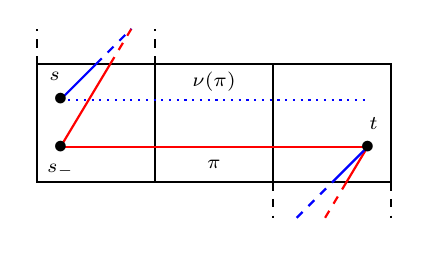
\begin{tikzpicture}[scale = 1.5]
      \node at (0,-0.5) {};
      \draw[thick] (0,0) rectangle (1,1);
      \draw[thick] (1,0) rectangle (2,1);
      \draw[thick] (2,0) rectangle (3,1);
      \draw[thick,dashed] (0,1) -- (0,1.3);
      \draw[thick,dashed] (1,1) -- (1,1.3);
      \draw[thick,dashed] (2,0) -- (2,-0.3);
      \draw[thick,dashed] (3,0) -- (3,-0.3);
      \draw[thick,red] (0.2,0.3) -- (2.8,0.3);
      \draw[thick,red] (0.2,0.3) -- (0.62,1);
      \draw[thick,red,dashed] (0.62,1) -- (0.8,1.3);
      \draw[thick,red,dashed] (2.62,0) -- (2.44,-0.3);
      \draw[thick,red] (2.62,0) -- (2.8,0.3);
      \draw[thick,blue,dotted] (0.2,0.7) -- (2.8,0.7);
      \draw[thick,blue] (0.2,0.7) -- (0.5,1);
      \draw[thick,blue,dashed] (0.5,1) -- (0.8,1.3);
      \draw[thick,blue,dashed] (2.2,-0.3) -- (2.5,0);
      \draw[thick,blue] (2.5,0) -- (2.8,0.3);
      \node at (2.8,0.3) {$\bullet$};
      \node at (0.2,0.3) {$\bullet$};
      \node at (0.2,0.7) {$\bullet$};
      \node at (1.5,0.85) {\scriptsize{$\nu(\pi)$}};
      \node at (1.5,0.15) {\scriptsize{$\pi$}};
      \node at (2.85,0.5) {\scriptsize{$t$}};
      \node at (0.2,0.1) {\scriptsize{$s_-$}};
      \node at (0.15,0.9) {\scriptsize{$s$}};
    \end{tikzpicture}
    \qquad\qquad
    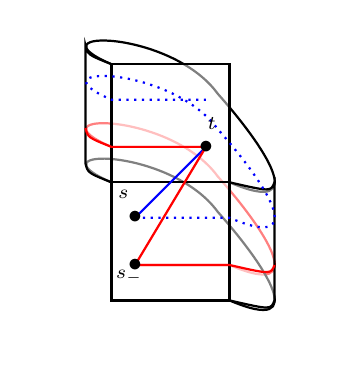
\begin{tikzpicture}[scale = 1.5]
      % \draw[] (1,1) .. controls (1.7,0.7) and (1.3,1.3) .. (0.9,1.75) .. controls (0.5,2.3) and (-0.7,2.3) .. (0,2);
      % \draw[] (1,0) .. controls (1.7,-0.3) and (1.3,0.3) .. (0.9,0.75) .. controls (0.5,1.3) and (-0.7,1.3) .. (0,1);
      \draw[thick,red] (0.2,0.3) -- (1,0.3)  .. controls (1.7,0.0) and (1.3,0.6) .. (0.9,1.05) .. controls (0.5,1.6) and (-0.7,1.6) .. (0,1.3) -- (0.8,1.3);
      \draw[thick,fill = gray!0,fill opacity=0.5] (1,0) .. controls (1.7,-0.3) and (1.3,0.3) .. (0.9,0.75) .. controls (0.5,1.3) and (-0.7,1.3) .. (0,1) -- (0,2) .. controls (-0.7,2.3)
      and (0.5,2.3) .. (0.9,1.75) .. controls (1.3,1.3) and (1.7,0.7) .. (1,1) -- (1,0);
      \draw[thick,fill = gray!0,fill opacity=0.5] (1,0) .. controls (1.35,-0.08) .. (1.38,0) -- (1.38,1) .. controls (1.35,0.92) .. (1,1) -- (1,0);
      \draw[thick,fill = gray!0,fill opacity=0.5] (0,1) .. controls (-0.2,1.08) .. (-0.22,1.16) -- (-0.22,2.16) .. controls (-0.2,2.08) .. (0,2) -- (0,1);
      % \draw[fill = gray!40,fill opacity=0.5] (1,0) -- (1.3,-0.1) -- (1.3,0.9) -- (1,1) -- (1,0);
      \draw[thick,fill = gray!0,fill opacity = 0.5] (0,0) rectangle (1,1);
      \draw[thick,fill = gray!0,fill opacity=0.5] (0,1) rectangle (1,2);
      \draw[thick,blue,dotted] (0.2,0.7) -- (1,0.7)  .. controls (1.7,0.4) and (1.3,1.0) .. (0.9,1.45) .. controls (0.5,2.0) and (-0.7,2.0) .. (0,1.7) -- (0.8,1.7);
      \draw[thick,blue] (0.2,0.7) -- (0.8,1.3);
      \draw[thick,red] (0.2,0.3) -- (0.8,1.3);
	\draw[thick,red] (0.2,0.3) -- (1,0.3) .. controls (1.35,0.22) .. (1.38,0.3);
	\draw[thick,red] (0.8,1.3) -- (0,1.3) .. controls (-0.2,1.38) .. (-0.22,1.46);
      \node at (0.8,1.3) {$\bullet$};
      \node at (0.2,0.3) {$\bullet$};
      \node at (0.2,0.7) {$\bullet$};
      \node at (0.85,1.5) {\scriptsize{$t$}};
      \node at (0.15,0.2) {\scriptsize{$s_-$}};
      \node at (0.1,0.9) {\scriptsize{$s$}};
    \end{tikzpicture}
  \end{center}
\end{figure}

It has three squares (look at the view on the left), and the bottom
face of the rightmost square is glued to the top face of the
leftmost one. The glueing is displayed on the right. Consider now $s$,
$s_-$ and $t$ as in the figure. $\tracep{X}{s}{t}$ has one connected
component (one of its element is drawn in plain blue) while
$\tracep{X}{s'}{t}$ has two (an element of each is drawn in plain
red).  Hence Lemma~\ref{lem:tech2} would fail if we allowed
$K$ to be a general non-looping precubical set, not just a cubical complex.

The argument we use to prove Lemma~\ref{lem:tech2} works
perfectly well in general non-looping precubical sets, except for one
thing: it may be that $\nu (\pi) (1)$ does not coincide with $t$, and
is strictly above.  See the dotted blue line in the figure above to
contemplate what $\nu (\pi)$ looks like in this example.


\subsection{Consequences}
	\subsubsection{Computability}
	
	This result has for consequence that our directed homology is computable in the sense that the following problem is decidable:
	\begin{itemize}
		\item[\textbf{data:}] Two cubical complexes $K$ and $K'$ and an integer $n \geq 1$.
		\item[\textbf{question:}] Are $\nathomolbw{n}{\digeom{K}}$ and $\nathomolbw{n}{\digeom{K'}}$ bisimilar when homology is with values in $\RR$-modules ?
	\end{itemize}
	
	For this, it is enough to compute $\nathomolbw{n}{K}$ and $\nathomolbw{n}{K'}$ in the reals and use the algorithm from the last chapter. Given a cubical complex, computing $\nathomolbw{n}{K}$ can be done in two steps:
	\begin{enumerate}
		\item compute a diagram with values in finite pre-simplicial sets (similar to precubical sets, or simplicial sets without degeneracies) from which the application of the simplicial homology functor produces a diagram in real vector spaces isomorphic to $\nathomolbw{n}{K}$,
		\item compute this homology.
	\end{enumerate}
	
	The second step is implemented in several classic tools for computing homology. For example:
	\begin{itemize}
		\item Sage module CHomP \cite{chomp},
		\item RedHom library \cite{redhom}.
	\end{itemize}
	
	For the first step, there are two possibilities:
	\begin{itemize}
		\item use the work from \cite{raussen10}. This produces a diagram in prod-simplicial complexes, kind of a mix between pre-cubical and pre-simplicial sets. From those prod-simplicial complexes, it is possible to produce pre-simplicial sets as required. We will not present the full construction from \cite{raussen10}, but at least develop an example. Consider the following d-space:
		\begin{figure}[H]
  \begin{center}
    	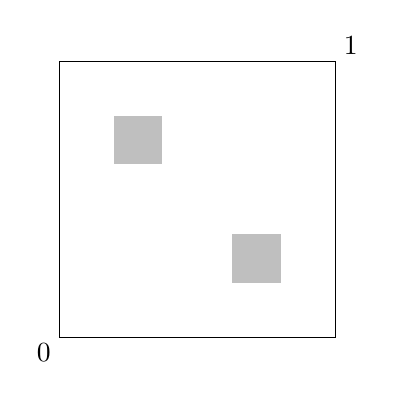
\begin{tikzpicture}[auto]
\draw (0,0) rectangle (3.5,3.5);
\draw [fill = gray!50,draw = gray!50] (0.7,2.2) rectangle (1.3,2.8);
\draw [fill = gray!50,draw = gray!50] (2.2,0.7) rectangle (2.8,1.3);
\node at (-0.2,-0.2) {$0$};
\node at (3.7,3.7) {$1$};

\end{tikzpicture}

  \end{center}
\end{figure}
It is the geometric realization of some cubical complex. To compute the prod-simplicial complex for the trace space between $0$ and $1$, we ``extend'' every holes in at least one direction and check which induced spaces have a non-empty trace space. For example, by extending each hole in one direction we obtain four cases:
	\begin{figure}[H]
  \begin{center}
    	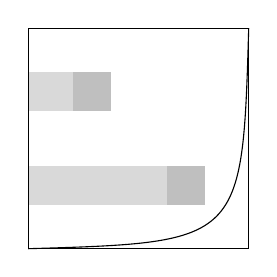
\begin{tikzpicture}[auto,scale=0.8]
\draw [fill = gray!50,draw = gray!50] (0.7,2.2) rectangle (1.3,2.8);
\draw [fill = gray!50,draw = gray!50] (2.2,0.7) rectangle (2.8,1.3);
\draw [fill = gray!30,draw = gray!30] (0,2.2) rectangle (0.7,2.8);
\draw [fill = gray!30,draw = gray!30] (0,0.7) rectangle (2.2,1.3);
\draw (0,0) .. controls (3.4,0.1) .. (3.5,3.5);
\draw (0,0) rectangle (3.5,3.5);
\end{tikzpicture}
\begin{tikzpicture}
\draw[color = white] (0,-1) rectangle (0.7,-2);
\end{tikzpicture}
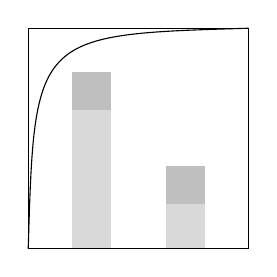
\begin{tikzpicture}[auto,scale=0.8]
\draw [fill = gray!50,draw = gray!50] (0.7,2.2) rectangle (1.3,2.8);
\draw [fill = gray!50,draw = gray!50] (2.2,0.7) rectangle (2.8,1.3);
\draw [fill = gray!30,draw = gray!30] (0.7,0) rectangle (1.3,2.2);
\draw [fill = gray!30,draw = gray!30] (2.2,0) rectangle (2.8,0.7);
\draw (0,0) .. controls (0.1,3.4) .. (3.5,3.5);
\draw (0,0) rectangle (3.5,3.5);
\end{tikzpicture}
\begin{tikzpicture}
\draw[color = white] (0,-1) rectangle (0.7,-2);
\end{tikzpicture}
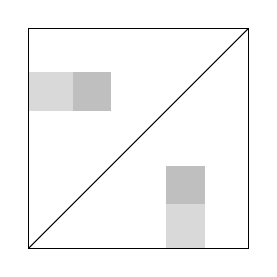
\begin{tikzpicture}[auto,scale=0.8]
\draw [fill = gray!50,draw = gray!50] (0.7,2.2) rectangle (1.3,2.8);
\draw [fill = gray!50,draw = gray!50] (2.2,0.7) rectangle (2.8,1.3);
\draw [fill = gray!30,draw = gray!30] (0,2.2) rectangle (0.7,2.8);
\draw [fill = gray!30,draw = gray!30] (2.2,0) rectangle (2.8,0.7);
\draw (0,0) -- (3.5,3.5);
\draw (0,0) rectangle (3.5,3.5);
\end{tikzpicture}
\begin{tikzpicture}
\draw[color = white] (0,-1) rectangle (0.7,-2);
\end{tikzpicture}
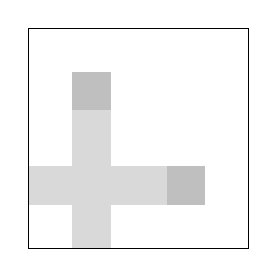
\begin{tikzpicture}[auto,scale=0.8]
\draw [fill = gray!50,draw = gray!50] (0.7,2.2) rectangle (1.3,2.8);
\draw [fill = gray!50,draw = gray!50] (2.2,0.7) rectangle (2.8,1.3);
\draw [fill = gray!30,draw = gray!30] (0.7,0) rectangle (1.3,2.2);
\draw [fill = gray!30,draw = gray!30] (0,0.7) rectangle (2.2,1.3);
\draw (0,0) rectangle (3.5,3.5);
\end{tikzpicture}

  \end{center}
\end{figure}
	Only three of them have non-empty trace spaces which produces three cells in the prod-simplicial complex. Those cells are all of dimension $0$ meaning that the trace space is equivalent to a 3 point space.
		\item the second possibility is to use the recent work from \cite{ziemianski17}. This produces a diagram in finite posets from which it is possible to construct the required diagram in presimplicial sets by applying the nerve functor. Those posets are produced by constructing the set of \textbf{cube chains}, which are very similar to our discrete traces. They are sequences of cubes such that the upper corner of a cube coincide with the lower corner of the next cube. They can essentially be ordered by inclusion, which produce the poset.
	\end{itemize}
	
	One should observe that classical methods from persistent homology cannot apply in our case, even multidimensional persistency \cite{zomorodian05}. The problem is that the quiver that we use (the categories $\tracebw{X}$ and $\tracehm{X}$) are not even tamed which makes the theory of persistency much harder.
	
	\subsubsection{Invariance under some action refinements}
	
	We have seen in Section \ref{subsec:actref} the particular importance of action refinement. Let us restrict here to the case of refining actions only by finite sequences of actions. Geometrically speaking, those refinements are modeled by \textbf{subdivision}. Given a cubical complex $K$, its subdivision $\subd{K}$ is the cubical complex whose cubes are $$\{(D,2x + \sum\limits_{j \in D'} \vec{1}_j) \mid (D,x) \in K, \, D' \subseteq D\}.$$
	
	It is clear that $\digeom{\subd{K}}$ is dihomeomorphic to $\digeom{K}$. Consequently, $\nathomolbw{n}{\digeom{K}}$ is isomorphic to $\nathomolbw{n}{\digeom{\subd{K}}}$. Hence:
	
	\begin{coro}[Invariance under sequential refinement]
	$\disnathomolbw{n}{K}$ is bisimilar to $\disnathomolbw{n}{\subd{K}}$.
	\end{coro}




\section{Relation with inessential equivalences, second homotopy axiom}
\label{sec:sechomax}

\subsection{Traces vs dipaths, again}

We argued in Section \ref{subsec:trpacat} the difference between traces and dipaths. We used dipaths to define equivalences because they are purer, in the sense that path-connected components of spaces of dipaths are exactly equivalence classes of dipaths modulo dihomotopy, which is not the case for trace spaces. On the contrary, trace spaces are better for computation: concatenation is associative which allows one to define nice structures like the category of traces, they are computable in easy case \cite{raussen10}. That is why we used traces instead of dipaths in the definition of our directed homologies. But we could have defined them using only dipaths and dihomotopies.

First, since the dipaths category is not strictly a category because concatenation is only associative modulo dihomotopy, we cannot use it instead of the trace category. But we can use the fundamental category $\funcat{X}$. We can then apply the enveloping category $\E$ and the category of factorizations $\mathcal{F}$ on it. Similarly to $\tracehm{X}$, we can define a functor $\map{\overrightarrow{BP}(X)}{\env{\funcat{X}}}{\hotop}$ which maps every pair of points $(a,b)$ to the space of dipaths $\dipp{X}{a}{b}$ and every extensions $(\tra{\alpha},\tra{\beta})$ to the homotopy class of the continuous function from $\dipp{X}{a}{b}$ to $\dipp{X}{a'}{b'}$ which maps a dipath $\gamma$ to $\alpha\star\gamma\star\beta$. Remember that, since concatenation is not associative, we must define everything modulo homotopy. Since homology is invariant under homotopy, meaning that the functor $H_n$ is actually a functor from $\hotop$ to $\modu{\R}$, one can define directed homology by applying this functor to $\overrightarrow{BP}(X)$. We denote the functor $H_{n-1}\circ\overrightarrow{BP}(X)$ by $\dipnathomolhm{n}{X}$. 

Everything that we have done with traces can be done with this definition with the following two exceptions: it is not possible to define diagrams of homotopy since we must point the dipath spaces and that we do not have a canonical dipath, but a dihomotopy class of dipaths ; the theory of homology of diagrams does not work well with this definition since $\dipnathomolhm{n}{X}$ cannot be defined as the homology of a chain complex of diagrams of modules (we should somehow have something modulo homotopy). The other annoying property is that, in general, $\dipnathomolhm{n}{X}$ is not bisimilar to $\nathomolhm{n}{X}$, since dipath spaces and trace spaces do not have the same homology. But, this is the case in cubical complexes:

\begin{prop}
For every cubical complexes $K$, $\nathomolhm{n}{\digeom{K}}$ is bisimilar to $\dipnathomolhm{n}{\digeom{K}}$.
\end{prop}


\begin{proof}
Let $X = \digeom{K}$. We construct an open map $\map{(\Phi,\sigma)}{\nathomolhm{n}{X}}{\dipnathomolhm{n}{X}}$ as follow:
\begin{itemize}
	\item the natural isomorphism is given by \cite{raussen09},
	\item $\Phi$ from $\env{\trace{X}}$ to $\env{\funcat{X}}$ which maps $(a,b)$ to $(a,b)$ and every extension $(\tra{\alpha},\tra{\beta})$ to $([\alpha],[\beta])$. It is trivially surjective on objects, and given an extension $([\alpha],[\beta])$ from $(a,b)$ to $(a',b')$, $(\tra{\alpha},\tra{\beta})$ is an extension from $(a,b)$ to $(a',b')$.
\end{itemize}
\end{proof}


\subsection{Second homotopy axioms}


Our goal is to prove the following:

\begin{theo}[Second homotopy axiom]
For every two cubical complexes $K$ and $K'$, if $\digeom{K}$ and $\digeom{K'}$ are inessentially equivalent, then their homology $\nathomolhm{n}{\digeom{K}}$ and $\nathomolhm{n}{\digeom{K'}}$ are bisimilar.
\end{theo}

This means that our directed homology is an invariant of inessential equivalences at least on spaces where we can do computations. By the previous proposition, it is enough to prove that $\dipnathomolhm{n}{\digeom{K}}$ and $\dipnathomolhm{n}{\digeom{K'}}$ are bisimilar. We can conclude using the following:

\begin{lemme}
If $(X,A)$ is a FIDR, and if $\map{H}{X}{\ine{X}}$ is the corresponding dihomotopy, then $H_1$ induces an open map from $\dipnathomolhm{n}{X}$ to $\dipnathomolhm{n}{A}$. Similarly, for PIDR.
\end{lemme}

\begin{proof}
First, the induced functor is defined $\map{\Phi_{H_1}}{\fac{\funcat{X}}}{\fac{\funcat{A}}}$ by sending every class $[\gamma]$ to $[H_1\circ\gamma]$. This functor is surjective since $H_1$ is the identity on $A$. It satisfies the fibrational property: given a class $[H_1\circ\gamma]$ of dipaths modulo dihomotopy in $A$ with $\gamma$ from $x$ to $y$ and let $([\alpha],[\beta])$ be an extension in $A$, i.e., $\alpha$ and $\beta$ are dipaths in $A$ with $\alpha$ from $x'$ to $H_1(x)$ and $\beta$ from $H_1(y)$ to $y'$.

By the last condition of a future deformation retract, there is a dipath $\alpha'$ in $X$ from $w$ to $x$ such that $H_1\circ\alpha'$ and $\alpha$ are dihomotopic.

$\dipp{X}{y}{y'}$ is non-empty since it contains $H(y)\star\beta$. Since $\map{H_1\circ\_}{\dipp{X}{y}{y'}}{\dipp{A}{H_1(y)}{y'}}$, $\delta \longmapsto H_1\circ\delta$ is a homotopy equivalence, $\map{H_1\circ\_}{\funcat{X}(y,y')}{\funcat{A}(H_1(y),y')}$, $[\delta] \longmapsto [H_1\circ\delta]$ is a bijection. There is, thus, a dipath $\beta'$ from $y$ to $y'$ such that $H_1\circ\beta'$ is dihomotopic to $\beta$.
Then $([\alpha'],[\beta'])$ is the lifting we were looking for.

Now, $H_1$ induces a natural transformation, $\map{\sigma_{H_1}}{\dip{X}}{\dip{A}\circ\Phi_{H_1}}$ by $\map{\sigma_{H_1,[\gamma]}}{\dipp{X}{x}{y}}{\dipp{A}{H_1(x)}{H_1(y)}}$, $\delta \longmapsto H_1\circ\delta$ which is a homotopy equivalence. Consequently, by applying the homology functor, this forms a natural isomorphism from $\dipnathomolhm{n}{X}$ to $\dipnathomolhm{n}{A}\circ\Phi_{H_1}$.
\end{proof}

\section*{Conclusion}

In this last chapter, we come full circle. Using bisimilarity to compare diagrams of homology makes all our theory coherent: the two definitions using natural systems and bimodules are equivalent; homotopy axioms works up to bisimilarity; for cubical complexes, diagrams of homology are computable up to bisimilarity; and finally, for cubical complexes, our homology is an invariant of inessential equivalence.





